
\begin{figure}[t]
    \begin{centering}
        % \subfloat[Some cool graphic]
        {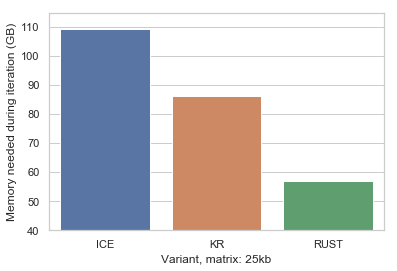
\includegraphics[scale=1]{figures/results/memiter_25}}
        \caption[Memory needs iterating 25kb]
        {\textbf{Memory needed during iteration} for correcting the 25kb matrix. Smaller is better.}
        \label{fig:memiter25}
\end{centering}
\end{figure}

\begin{figure}[t]
    \begin{centering}
        \subfloat[Available data]
        {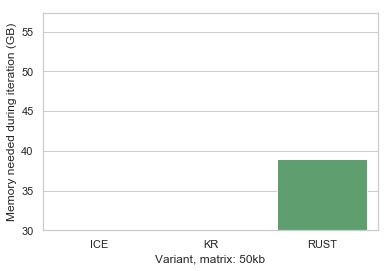
\includegraphics[scale=0.5]{figures/results/memiter_50}}
        \subfloat[Extrapolated data]
        {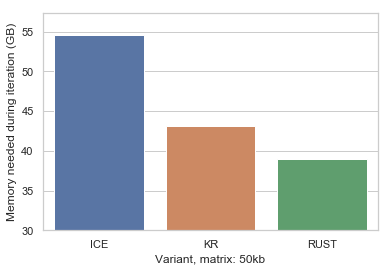
\includegraphics[scale=0.5]{figures/results/memiter_50_extra}}
        \caption[Memory needs iterating 50kb]
        {\textbf{Available and Extrapolated Data about Memory needed during
        iteration} of the 50kb matrix. Rust value is accurate, values for ICE
        and KR are not accurately available, but have been observed to be in
        the extrapolated areas. Smaller is better.}
        \label{fig:memiter50}
    \end{centering}
\end{figure}



